\documentclass[a4paper,10pt]{article}

%\usepackage[italian]{babel}
%\usepackage[latin1]{inputenc}
\usepackage{graphicx}
\usepackage{url}

%opening

\begin{titlepage}
 \title{PasCaml}
\author{Riccardo M. Cefal\`a \\Flavio Vella}
\end{titlepage} 
\begin{document}

\maketitle

\begin{abstract}
L'obiettivo del progetto \`e stato quello di realizzare in Ocaml un interprete 
per un sottinsieme del Linguaggio Pascal per il corso di Programmazione
Avanzata.
Per far ci\`o \`e stato inizialmente
definito il sottoinsieme del liguaggio Pascal da rappresentare (PasCaml)  e 
successivamente si \`e reso necessario sviluppare degli strumenti sia per la
analisi del codice sorgente in PasCaml (analizzatore lessicografico) sia
strumenti per il parsing tra la grammatica di linguaggio, da noi definita, e la
logica dell'interprete vera e propria.
\end{abstract}

\section{Analisi del progetto}
La prima scelta, in fase progettuale, \`e stata quella di stabilire la 
modalit\`a di lavoro dell'interprete: batch o interactive. Per semplicit\`a ci
siamo orientati verso una soluzione batch per semplificare l'analisi
lessicografica. In secondo luogo abbiamo definito il sottoinsieme di Pascal da
rappresentare (tipi, costrutti, operatori e quant'altro) nel modo che segue:
\begin{itemize}
 \item Tipi = \verb|{ integer , real }|
 \item Operatori = \verb|{ +, /, *, -, =, <, >, <>, >=, <=, and, or }|
 \item Controlli di flusso = \verb|{ if, while }|
 \item Routine = \verb|{ procedure }|
\end{itemize}
Infine sono state definite tutte le altre parole chiave riservate al linguaggio
che ne identificano la struttura. In particolare, nella nostra idea progettuale
il workflow dell'interprete PasCaml prevede:
\begin{enumerate}
 \item Un file scritto in PasCaml viene passato come argomento all'interprete.
 \item Tale file viene analizzato dall'analizzatore lessicografico che 
restituisce le parole chiave e le parole che reppresentano identificatori (nome
di variabili e nomi di procedure) sotto forma di token.
 \item L'output ritornato dall'analizzatore lessicografico viene parsato 
(analisi sintattica); in questa fase viene verificata che la grammatica del file
sorgente corrisponda a quella definita nel parser.
 \item Se il passo precedente ha esito positivo allora viene fatto il matching 
tra il parser e la logica dell'inteprete e viene eseguito il codice in input
altrimenti viene sollevata un'eccezione sul parsing.
\end{enumerate}
 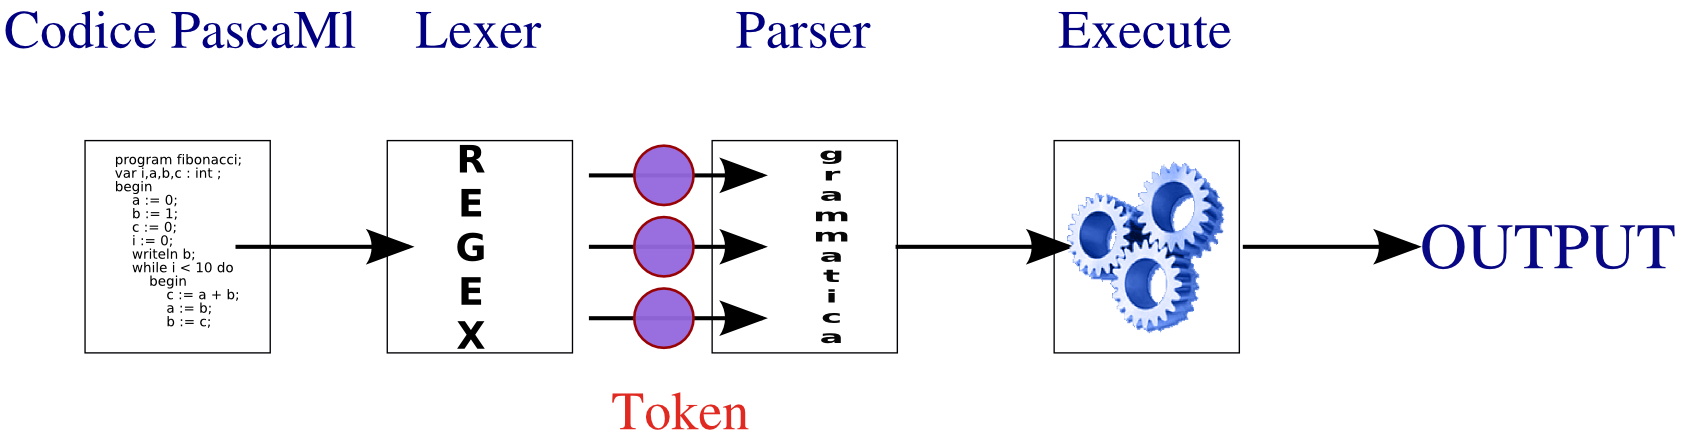
\includegraphics[scale=0.25]{./pics/pascaml01.png}


\section{Analisi lessicografica}
Un analizzatore lessicografico, chiamato anche lexer, \`e la parte di programma 
che analizza un testo in ingresso, ovvero uno stream di caratteri, e produce
come output un insieme di blocchi di testo categorizzati, chiamati token.
Quindi il compito di un lexer, in sintesi, \`e leggere dei lessemi (definizione
formale dei token) e suddividerli in categorie (tramite espressioni regolari)
attribuendo loro il significato associato.
Un analizzatore lessicografico in OCaml pu\`o essere implementato sfruttando il 
tool \textit{OCamlLex}.
Tale tool produce dei token a partire da un set di espressioni regolari alle 
quali sono associte delle azioni semantiche.


\subsection{Ocamllex}
Questo tool, similmente al programma lex di Unix, permette di descrivere con una
 sintassi semplice un lexer: l'implementazione di lex utilizza la sintassi del
linguaggio C, mentre OCamlLex utilizza la sintassi di OCaml. Per scrivere un
analizzatore sintattico con OCamlLex bisogna:

\begin{itemize}
\item scrivere il file sorgente nel formato riconosciuto da OCamlLex 
(con estensione .mll)
\item passare questo file ad OCamlLex che produce il file sorgente OCaml ”puro” 
che pu\`o essere compilato ed eseguito.
\end{itemize}

Il file di input per OCamlLex \`e un Lexer ML, cio\`e un file Lexer ma che nelle
 azioni da compiere usa istruzioni OCaml.Esso \`e composto da 4 parti:
\begin{description}
\item [intestazione] che contiene il codice che viene eseguito prima
dell' effettiva analisi lessicale; serve ad importare moduli aggiuntivi, a
definire tipi di dato e variabili utilizzabili dal lexer
\item [definizioni] dove possiamo dichiarare variabili che facilitano la 
leggibilit\`a delle espressioni regolari
\item [regole] la parte centrale del lexer che si occupa dell’analisi: \`e 
composta da alcune regole, che associano un pattern (definito tramite
espressioni regolari) ad una certa azione; questa azione pu\`o consistere nella
restituzione di un token (come nel nostro caso) ma in generale pu` contenere una
qualunque sequenza di istruzioni OCaml
\item [coda] che contiene il codice che viene eseguito dopo l’analisi lessicale,
 se necessario.
\end{description}


\subsection{Implementazione}
Il primo passo fatto nello sviluppare il lexer \`e stato quello di definire i 
simboli del nostro linguaggio cio\`e definire tutte quelle parole a cui vogliamo
attribuire un significato semantico univoco (lessemi e token come abbiamo detto
in precedenza). Nello specifico abbiamo definito:
\begin{itemize}
 \item letterali numerici: \`e l'insieme delle stringhe numeriche 
rappresentate dai token \verb|L_INT| e \verb|L_REAL|
\end{itemize}
L'insieme delle stringhe numeriche, per gli \verb|L_INT|, \`e ottenuto 
tramite l'espressione regolare \textit{'-'?['0'-'9']+ as l}, mentre l'azione
associata \textit{\{ L\_INT(int\_of\_string l) \}} estrae un oggetto di tipo
intero dalla sua rappresentazione letterale.
Quanto detto pu\`o essere analogamente affermato per il token \verb|L_REAL|.

\begin{itemize}
 \item simboli e operatori : \`e l'insieme dei caratteri che rappresentano i 
simboli e gli operatori del liguaggio come ad esempio \verb|{ ``+''|,
\verb|``:=''|, \verb|``;''|, \verb|``(''|, \verb|``and'' }|, i quali sono
associati rispettivamente ai seguenti token: \verb|PIU|, \verb|ASS|,
\verb|PVIRG|, \verb|SPAREN| e \verb|AND|.
\end{itemize}
\begin{itemize}
 \item keywords : \`e l'insieme delle stringhe che rappresentano le parole 
chiave riservate al liguaggio
per esempio ``\texttt{begin}'', ``\texttt{if}'', ``\texttt{integer}'',
``\texttt{procedure}'' associati 
ai rispettivi token: \verb|BEGIN|, \verb|IF|, \verb|INTEGER|, \verb|PROCEDURE|.
\end{itemize}
\begin{itemize}
 \item built-in : sono particolari keywords ai quali viene associata una 
particolare funzione.
Questo insieme \`e composto dalle stringhe ``write'' e ``writeln'' alle quali 
sono associati i seguenti token rispettivamente \verb|WRITE| e \verb|WRITELN|.
\end{itemize}
\begin{itemize}
 \item identifier : \`e l'insieme delle stringhe alfanumeriche che iniziano per 
letterale reppresentato dal token \verb|IDENTIFIER|.
\end{itemize} 
L'espressione regolare che rappresenta tutti i possibili \verb|identifier| \`e
\begin{center}
 \textit{['a'-'z''A'-'Z']['a'-'z''A'-'Z''0'-'9']*}.
\end{center}
OCaml consente la definizione di tipi con pi\`u costruttori;
OCamlLex, in congiunzione a OCamlYacc (di cui si parler\`a nel prossimo 
paragrafo) sfrutta questa caratteristica per gestire la rappresentazione dei
token e semplificarne la gestione da parte del parser.
In particolare ogni azione associata ai lessemi costruisce un oggetto di tipo 
\verb|token| tramite il costruttore di tipo corrispondente al lessema stesso.
Nel nostro caso, alcuni dei costruttori del tipo \verb|token| necessitano di 
un argomento; in particolare per il costruttore del token \verb|IDENTIFIER|
l'argomento \`e la stringa stessa , analogamente, per i costruttori dei token
\verb|L_INT| e \verb|L_REAL| l'argomento \`e rispettivamente un intero e un
float.

In conclusione possiamo riassumere il workflow di lexer nel modo seguete:
\begin{enumerate}
\item Riceve in input un file di testo scritto in PasCaml.
\item Genera delle sequenze di token filtrando il testo tramite espressioni 
regolari.
\item Solleva un errore lessicografico se esiste almeno una parola o un 
carattere non definito dalle espressioni regolari.
\item Passa al parser la sequenza dei token se l'esito del passo precedente \`e 
andato a buon fine.
\end{enumerate}

\section{Parser}
I semplici token riconosciuti tramite l'analizzatore lessicografico,
organizzati in sequenze definiscono costrutti pi\`u complessi che rappresentano
le \textit{frasi} del linguaggio e che assumeranno differenti significati per
l'interprete.

Il parser ha il compito di riconoscere tali sequenze, assicurare che esse siano
conformi alle regole sintattiche che definiscono il linguaggio (regole di
produzione) e popolare le strutture dati che verranno utilizzate
dall'interprete.

Pi\`u in generale ed in estrema sintesi si può affermare che un
linguaggio di
programmazione imperativo \`e un formalismo attraverso il quale si possono
rappresentare comandi per un operatore che esegue operazioni su dati.

Il risultato delle operazioni svolte dal parser sar\`a di fatto la traduzione
del testo in un ``meta-linguaggio'' comprensibile al suddetto operatore (il
nostro interprete), composto da rappresentazioni di \textit{espressioni} (i
dati) e \textit{comandi} (le istruzioni).

\subsection{OCamlYacc}
La scrittura di un parser da zero pu\'o essere un compito molto arduo senza uno
strumento come OCamlYacc. Questo software, similmente al programma yacc di Unix
, permette di descrivere con una sintassi semplice un parser: l'implementazione
 di yacc utilizza la sintassi del linguaggio C, mentre OCamlYacc utilizza la
 sintassi di OCaml.
I passi per sviluppare un parser sono i seguenti:
\begin{itemize}
    \item specificare la grammatica del linguaggio che si vuole usare nella
forma riconosciuta da OCamlYacc: per ogni regola grammaticale definiamo 
un'azione.
    \item scrivere un analizzatore lessicale che processi il file di input e
passi i token riconosciuti al parser (il lexer)
    \item compilare entrambi i file con i rispettivi tool per ottenere un
parser completo
\end{itemize}
Il file di descrizione della grammatica per OCamlYacc \`e composto da 4 parti:
\begin{description}
\item[intestazione] che contiene il codice che viene eseguito prima 
dell'effettiva analisi; serve ad importare moduli aggiuntivi, a definire tipi
di dato e variabili utilizzabili dal lexer e dal parser stesso.

\item[dichiarazioni] dove definiamo i simboli terminali e non terminali
utilizzpi\`uella grammatica (questi corrispondono a quelli riconosciuti dal
lexer, pi\`u quelli necessari all'analisi semantica); vengono dichiarati 
anche i tipi di dati corrispondenti ai valori dei simboli, 
la loro associativit\`a ed altre caratteristiche.

\item[regole] regole grammaticali che consistono in produzioni che vanno da un
simbolo non terminale a elementi pi\`u ``atomici'' e che sono riconosciuti dal
parser.

\item[coda] che contiene il codice che viene eseguito dopo l'analisi, questa
parte \`e opzionale.
\end{description}

\subsection{Strutture e tipi di dato}
Il meta-linguaggio al quale si \`e accennato nell'introduzione di questo 
paragrafo \`e in realt\`a costituito da apposite strutture dati. 
Di seguito verranno esaminate tali strutture dati, definite per 
rappresentare espressioni e istruzioni.

\subsubsection{Espressioni}
Generalmente, si pu\'o scomporre un'espressione in sotto-espressioni fino a
raggiungere i suoi elementi atomici costituitvi. Nel nostro caso le espressioni
si limiteranno a rappresentare valori numerici ottenuti a partire da letterali
numerici, identificatori e operazioni.
Sono dunque questi gli elementi che costituiscono le espressioni.

\paragraph{Letterali numerici}
Il tipo di dato \verb|num| consente di rappresentare i tipi ``integer'' e
``real'' del pascal:
\begin{verbatim}
 type num = Int of int | Real of float
\end{verbatim}

\paragraph{Identificatori}
L'insieme degli identificatori validi \`e un sottoinsieme del tipo \verb|string|
di Ocaml. \`E quindi gi\`a adeguato a rappresentarli. Gli identificatori sono
impiegati per designare variabili o nomi di procedure.

\paragraph{Operazioni}
La maggior parte degli operatori sono di tipo di binario, ovvero le
operazioni che rappresentano sono costituite dalle sotto-espressioni che
compaiono a destra e a sinistra dell'operatore. La loro definizione \`e dunque
ricorsiva poich\'e un'operazione \`e a sua volta un'espressione.
Il risultato d'insieme \`e illustrato dalla definizione del tipo \verb|expr|
che include, oltre alle operazioni anche i letterali numerici e gli
identificatori:\\

\verb|type expr =|
\begin{center}
\begin{tabular}{l l}
    \verb|And   of expr * expr|	& \verb|(* and booleano *)| \\
    \verb#| Div   of expr * expr# & \verb|(* divisione *)| \\
    \verb#| Ug    of expr * expr#& \verb|(* uguaglianza *)| \\
    \verb#| Mau    of expr * expr#& \verb|(* maggiore uguale *)| \\
    \verb#| Ma    of expr * expr#& \verb|(* maggiore *)| \\
    \verb#| Ident of string#	&\verb|(* identificatore *)| \\
    \verb#| Miu    of expr * expr#&\verb|(* minore uguale *)| \\
    \verb#| Mi    of expr * expr#&\verb|(* minore di *)| \\
    \verb#| Meno of expr * expr#&\verb|(* sottrazione *)| \\
    \verb#| Nu    of expr * expr#&\verb|(* diverso *)| \\
    \verb#| Neg   of expr#	&\verb|(* negato *)|\\
    \verb#| Num   of num#	&\verb|(* letterale numerico *)|\\
    \verb#| Or    of expr * expr#&\verb|(* or booleano *)|\\
    \verb#| Piu  of expr * expr#&\verb|(* addizione *)|\\
    \verb#| Per of expr * expr#&\verb|(* moltiplicazione *)|\\
\end{tabular}
\end{center}

I seguenti esempi mostrano le rappresentazioni tramite il tipo \verb|expr| di
alcune espressioni:\\
\begin{center}
\begin{tabular}{|l|l|}
\hline
\verb|3| & \verb|(Int 3)| \\
\hline
\verb|0.3| & \verb|(Real 0.3)| \\
\hline
\verb|x| & \verb|(Ident "x")| \\
\hline
\verb|0.3 * x| & \verb|Per((Real 0.3), (Ident x))| \\
\hline
\verb|(0.3 * x) + y| &
\verb|Piu(Per((Real 0.3), (Ident x)), (Ident y))| \\
\hline
\end{tabular} 
\end{center}

\subsubsection{Istruzioni}
Similmente alle espressioni anche per le istruzioni \`e stato creato un tipo di
dato in grado di rappresentare non solo una singola istruzione ma una sequenza
di esse. Anche questa definizione \`e dunque in parte ricorsiva:

\begin{verbatim}
 type stmt =
     Assign of string * expr
    | Dumpenv of unit
    | If of expr * stmt * stmt
    | Procedure of string * expr list
    | Seq of stmt * stmt
    | Void of unit
    | While of expr * stmt
    | Write of expr
    | Writeln of expr
\end{verbatim}
Si pu\'o notare come la definizione dei costruttori ricalchi la struttura delle
istruzioni:
\begin{description}
 \item[Assign] Nel caso dell'assegnamento, il primo elemento della
coppia \verb|(string * expr)| rappresenta l'identifier a sinistra dell'operatore
``\verb|:=|'', mentre il secondo l'espressione alla sua destra.

\item[If] In modo del tutto simile una tripla del tipo 
\verb|(expr * stmt * stmt)| pu\'o rappresentare un'istruzione
``if...then...else'': il primo elemento \`e l'espressione da valutare, il
secondo \`e l'istruzione da eseguire per il ramo ``then'' e il terzo quella per
il ramo ``else''.

\item[Procedure] La chiamata di procedura \`e rappresentata attraverso una
coppia \verb|(string * expr list)| dove il primo elemento \`e il nome della
procedura e la lista di espressioni al secondo elemento sono i parametri.

\item[Seq] Sequenze di istruzioni possono essere rappresentate attraverso il
costruttore ricorsivo \verb|Seq|. Una sequenza di due istruzioni \`e
rappresentata come \verb|Seq(stmt, stmt)|, tre istruzioni come
\verb|Seq(stmt, Seq(stmt, stmt))| e cos\'i via.

\item[Void] Rappresenta lo statement vuoto, quindi non ha elementi.

\item[While] Una coppia \verb|(expr * stmt)| \`e in grado di rappresentare la
guardia e il corpo di un'istruzione while.

\item[Write e Writeln] Vengono impiegate per rappresentare le istruzioni che
stampano sullo standard output un'espressione \verb|expr|. Sebbene in PASCAL
tali istruzioni non sono integrate nel linguaggio, per semplicit\`a in PasCaml
verranno gestite come tali.

\item[Dumpenv] Istruzione ``diagnostica'' che verr\`a esposta in seguito.
\end{description}


La tabella che segue riporta alcuni esempi di
rappresentazione di istruzioni attraverso il tipo \verb|stmt|:

\begin{center}
\begin{tabular}{|l|l|}
\hline
\verb|a := 3| & \verb|Assign ("a", (Int 3))| \\
\hline
\verb|while 1 do write a| &
 \verb|While((Int 1), Write((Ident a)))| \\
\hline
\verb|a := 3;|\\ \verb|while 1 do write a| &
 \verb|Seq(Assign(...), While(...))|\\
\hline
\end{tabular} 
\end{center}

\subsubsection{Ambienti}
L'insieme di variabili, procedure e istruzioni definisce l'ambiente di un
programma PasCaml. Per rappresentare un ambiente \`e stato definito il tipo di
dato \verb|env|:
\begin{verbatim}
type env = {
    mutable idlist : (string * num) list;
    mutable proclist : (string * (string * num) list * env) list;
    mutable stmts : stmt;
}
\end{verbatim}
Il campo lista ``idlist'' contiene le coppie (identificatore, valore) che
designano le
variabili. Il campo ``stmts'' rappresenta le istruzioni da eseguire. Il campo
``proclist'' contiene una lista di triple ognuna delle quali rappresenta una
procedura. Le triple sono della forma (identificatore procedura, lista dei
parametri formali, ambiente della procedura).

\subsection{Parsing delle Espressioni}
Il meccanismo di parsing delle espressioni viene definito tramite le regole di
produzione del parser. Poich\'e vi sono vincoli di precedenza da rispettare 
per gli operatori, \`e stato necessario suddividere le regole di produzione in
modo da garantire che la loro appilicazione avvenisse in accordo a tali
vincoli.
La porzione del file parser.mly in cui \`e definito il parser riportato di
 seguito mostra le regole di produzione per le espressioni:
\begin{verbatim}
[...]
%token <int> L_INT
%token <float> L_REAL
%token <string> IDENTIFIER
[...]
identifier : IDENTIFIER { $1 } ;
[...]
expression:
     expr2 { $1 }
   | expr2 UG expr2  { Ug ($1,$3) }
   | expr2 NU expr2  { Nu ($1,$3) }
   | expr2 MAU expr2 { Mau ($1,$3) }
   | expr2 MA expr2  { Ma ($1,$3) }
   | expr2 MIU expr2 { Miu ($1,$3) }
   | expr2 MI expr2  { Mi ($1,$3) }
   ;

expr2:
    expr3 { $1 }
    | expr2 PIU expr3 { Piu ($1,$3) }
    | expr2 MENO expr3 { Meno ($1,$3) }
    | expr2 OR expr3 { Or ($1,$3) }
    ;

expr3:
    expr4 { $1 }
    | expr3 PER expr4 { Per ($1,$3) }
    | expr3 DIV expr4 { Div ($1,$3) }
    | expr3 AND expr4 { And ($1,$3) }
    ;

expr4:
    PIU expr4 { $2 }
    | MENO expr4 { Neg $2 }
    | SPAREN expression DPAREN { $2 }
    | number { $1 }
    ;

number:
    L_INT { Num (Int $1)  }
    | L_REAL { Num (Real $1) }
    | identifier { Ident $1 }
    ;
[...]
\end{verbatim}
La regola \texttt{identifier} estrae il valore dal token IDENTIFIER attraverso
il simbolo posizionale ``\$1'' che rappresenta il contenuto del primo
elemento 
nella regola (in questo caso IDENTIFIER) e poich\'e nella porzione delle
dichiarazioni il token IDENTIFIER \`e tipizzato in modo da essere una stringa,
il contenuto della produzione \texttt{identifier} sar\`a appunto una stringa.

Esso verr\`a utilizzato insieme ai token L\_INT e L\_REAL per rappresentare gli
elementi atomici delle espressioni nella produzione \texttt{number}.

Nella produzione \texttt{expr4} vi sono gli operatori che generano espressioni 
a pi\`u alta priorit\`a e che verranno adoperate dal parser ``prima'' delle
regole \texttt{expr3}, \texttt{expr2} ed \texttt{expression}. Tale priorit\`a
\`e garantita dal fatto che in quest'ultime regole compaiono in modo
gerarchico le espressioni di priorit\`a superiore che quindi devono essere
necessariamente valutate per completare la produzione.

Salendo per la catena di produzioni gli oggetti restituiti vengono combinati in
espressioni via via pi\`u complesse utilizzando i costruttori del tipo 
\verb|expr| a partire dai token che rispettano la regola \texttt{number}.

\subsection{Parsing delle Istruzioni}
In modo simile alle espressioni il parser riconosce i vari tipi di istruzioni e 
ne costruisce la rappresentazione impiegando i costruttori del tipo \verb|stmt|.
\begin{verbatim}
[...]
sezione_statement :
    | statement_composto { $1 } 
    ;

statement_composto :
    BEGIN statement_sequenza END { $2 } 
    | statement { $1 }
    ;

statement_sequenza : 
    statement_sequenza PVIRG statement { Seq ($1,$3) }
    | statement { $1 }
    ;

statement : 
    { Void () }
    | assegnamento_statement { $1 }
    | if_statement { $1 }
    | while_statement { $1 }
    | write_statement { $1 }
    | procedure_statement { $1 }
    | dumpenv_statement { $1 }
    ;

assegnamento_statement : 
    identifier ASS expression { Assign ($1,$3) }
    ;
[...]
\end{verbatim}

Per brevit\`a nel listato precedente non sono riportate tutte le produzioni per
le istruzioni. Si pu\'o tuttavia osservare la costruzione di un'istruzione di
assegnamento a partire da un \textit{identifier} e una \textit{expression}
attraverso la regola \textit{assegnamento\_statement}. Le istruzioni composte,
ovvero le sequenze di istruzioni contenute in \texttt{BEGIN...END}, vengono
costruite tramite applicazioni successive del costruttore \texttt{Seq}, come
mostrato nei precedenti paragrafi.

\subsection{Parsing degli Ambienti}
I programmi PASCAL sono ben strutturati in sezioni, il nostro
linguaggio semplificato prevede soltanto: 
\begin{itemize}
 \item la sezione di dichiarazione delle variabili.
 \item la sezione di dichiarazione delle procedure.
 \item la sezione delle istruzioni.
\end{itemize}
Questi tre elementi costituiscono un \textbf{blocco}: 
\begin{verbatim}
blocco:
    sezione_variabili
    sezione_procedure
    sezione_statement { {idlist = $1 ; proclist = $2 ; stmts = $3} }
    ;
\end{verbatim}
Ciascuna delle tre sezioni contemplate pu\'o essere eventualmente vuota.
Come si vede dalla regola di produzione \texttt{blocco} sopra illustrata e
ricordando la definizione del tipo \texttt{env}, a livello logico ogni blocco si
traduce in un ambiente, ovvero un oggetto \texttt{env}.

La seguente porzione di codice mostra un'esempio di definizione di blocco:
\begin{verbatim}
var a,b:int;

procedure p1 (x:int);
    var k:int;
    b := b + x;

begin
  a := 1;
  p1(a);
  write b
end
\end{verbatim}

La traduzione a livello logico svolta dall'azione combinata di parser e lexer
avr\`a come risultato l'oggetto di tipo \texttt{env} mostrato di seguito:
\begin{verbatim}
{
 idlist = [(a, (Int 0)); (b, (Int 0))];
 proclist = [ ("p1", [(x, (Int 0))], {
                                     idlist = [("k", (Int 0))]
                                     proclist = []
                                     stmts = Assign("b", exp);
                                    }) ];
 stmts = Seq(Seq(Assign("a", Num (Int 1)),Procedure("p1",["x"]),
        (Write "b"))
}
\end{verbatim}

Come si pu\'o notare ogni definizione di procedura, contenuta nella lista
funlist, contiene a sua volta l'ambiente della procedura stessa.
Poich\'e esso \`e un ambiente completo per ogni procedura \`e possibile
definire oltre a variabili e istruzioni anche sotto procedure. L'esempio
risulta pi\`u chiaro tenendo in considerazione le definizioni dei tipi di
descritte in questo paragrafo.

\subsection{Verso l'Interpretazione}
Come si \`e accennato il compito del parser \`e quello di fornire una
rappresentazione comprensibile all'interprete del codice PasCaml. Poich\'e il
risultato dell'esecuzione del nostro parser \`e un oggetto \texttt{env}, esso
rappresenter\`a l'astrazione dell'intero programma da passare all'interprete.

Tutte le regole di produzione culminano nella regola \texttt{program}:

\begin{verbatim}
program :
    | EOF { printf "File Vuoto!\n" ; raise End_of_file }
    | program_intestazione PVIRG blocco PUN  { 
        global_enviroment.enviroments <- [$3] ;
        execute_global global_enviroment.enviroments ;
        raise End_of_file }
    ;

program_intestazione :
    PROGRAM identifier { $2 }
    ;

\end{verbatim}

Al termine del parsing di tutte le componenti del programma, l'env generato
viene inserito in testa ad una lista di ambienti. L'interprete, attraverso la
funzione \texttt{execute\_global} estrarr\`a gli statement che verranno
eseguiti sequenzialmente.

\section{Logica dell'interprete}
A questo punto l'interprete \`e in grado di comprendere il programma la cui
rappresentazione viene inserita in una apposita pila definita nel modo seguente:
\begin{verbatim}
 type global = {
    mutable enviroments : env list;
}

let global_enviroment = {
    enviroments =  
        [{ idlist = [] ; proclist = [] ; stmts = (Void ()) }]
}
\end{verbatim}
e inizializzata con un ambiente ``vuoto''. La sequenza di azioni intraprese
dall'interprete da questo punto in poi \`e totalmente dipendente dalle
funzioni \texttt{execute} e \texttt{evaluate} che costituiscono il nucleo della
logica dell'interprete.


\subsection{La funzione evaluate}
La funzione \texttt{evaluate} consente la valutazione delle espressioni, ovvero
la loro risoluzione attraverso chiamate alle relative funzioni di somma,
prodotto, divisione, ecc. fino a ridurre l'espressione di partenza in un oggetto
non ulteriormente riducibile di tipo \texttt{num}. Il listato
seguente mostra l'implementazione di \texttt{evaluate}.
\begin{verbatim}
 let evaluate expression =  
    let rec aux = function
        And (e1, e2)  -> _and (aux e1, aux e2)
        | Div (e1, e2) -> _div (aux e1, aux e2)
        | Ug (e1, e2) -> _ug (aux e1, aux e2)
        | Mau (e1, e2) -> _mau (aux e1, aux e2)
        | Ma (e1, e2) -> _ma (aux e1, aux e2)
        | Ident s -> get_value s
        | Miu (e1, e2) -> _miu (aux e1, aux e2)
        | Mi (e1, e2) -> _mi (aux e1, aux e2)
        | Meno (e1, e2) -> _meno (aux e1, aux e2)
        | Nu (e1, e2) -> _nu (aux e1, aux e2)
        | Neg e -> _neg (aux e)
        | Num n -> n
        | Or (e1, e2) -> _or (aux e1, aux e2)
        | Piu (e1, e2) -> _piu (aux e1, aux e2)
        | Per (e1, e2) -> _per (aux e1, aux e2)
    in aux expression
\end{verbatim}
Tale funzione genera una sequenza di chiamate ricorsive a funzioni tra
loro molto simili, che per la maggior parte differiscono tra loro solo
per l'operatore applicato. Ad esempio, la funzione che esegue la somma di
 due \texttt{num} \`e definita come segue:
\begin{verbatim}
 let _piu = function
    ((Int a), (Int b)) -> (Int (a + b))
    |((Real a), (Real b)) -> (Real (a +. b))
    |((Real a), (Int b)) -> (Real (a +. (float_of_int b)))
    |((Int a), (Real b)) -> (Real ((float_of_int a) +. b))
\end{verbatim}
Poich\'e ogni funzione di questo tipo restituisce ancora un \texttt{num}, esse
possono essere passate come parametri di ulteriori funzioni, in modo da
ricalcare fedelmente la rappresentazione del tipo \texttt{expr}

Inoltre, l'esecuzione di un'istruzione che contiene un espressione deve essere
necessariamente preceduta dalla fase di valutazione dell'espressione. Ci\`o
rende la funzione \texttt{evaluate} di fondamentale importanza per l'interprete.

\subsection{La funzione execute}
La funzione \texttt{execute} \`e la funzione pi\`u importante dell'interprete.
Essa infatti, dato un oggetto \texttt{stmt} che rappresenta le istruzioni da
eseguire, completa le azioni corrispondenti al tipo di istruzione tramite 
chiamate ricorsive che terminano con l'effettiva esecuzione di funzioni 
definite all'interno dell'interprete. Tali funzioni svolgono le azioni
corrispondenti agli statement pi\`u semplici. Di seguito \`e riportata la
funzione \texttt{statement}:
\begin{verbatim}
 let execute statement =
    let rec exec = function
        Void unit -> unit
        | Seq (st1, st2) -> exec(st1) ; exec(st2)
        | Assign (id, exp) -> (assign id exp)
        | While (exp, st1) as whst ->
                if bool_eval exp then (exec(st1) ; exec(whst)) else ()
        | Write exp -> printf "%s " (string_of_num (evaluate exp))
        | Writeln exp -> printf "%s\n" (string_of_num (evaluate exp))
        | If (exp, st1, st2) ->
                if bool_eval exp then exec(st1) else exec(st2)
        | Procedure (id, par) ->
                global_enviroment.enviroments <-
                 (init_procedure_env id par)::global_enviroment.enviroments;

                exec (List.hd global_enviroment.enviroments).stmts ;

                global_enviroment.enviroments <- 
                 List.tl global_enviroment.enviroments ;

        | Dumpenv unit -> dump_env global_enviroment
    in exec statement
\end{verbatim}
Il listato precedente mostra come da uno statement pi\`u strutturato la funzione
\texttt{execute} chiama ricorsivamente se stessa fino a raggiungere statement
che operano sui dati o svolgono azioni reali. Essi sono soltanto gli
assegnamenti (Assign) e le stampe a video (Write, Writeln, Dumpenv).
In particolare per un assegnamento, la funzione \texttt{assign} cerca
l'identifier nello stack degli enviroment e se lo trova valuta l'espressione e
ne sostituisce il valore ad esso associato. Altrimenti solleva un'eccezione di
tipo \texttt{Identifier\_not\_found}.

Un'istruzione di controllo di flusso invece, non modifica direttamente i dati 
ne causa effetti collaterali (come la stampa a video). Ad esempio, nel caso del
 While tutto ci\`o che avviene \`e la valutazione dell'espressione guardia del 
while e, se essa \`e vera, viene eseguito lo statement che ne rappresenta
il corpo. Successivamente viene rieseguita la medesima istruzione While appena
terminata, in modo da rivalutare l'espressione ed eventualmente rieseguire il
corpo dell'istruzione.

\subsection{Gestione degli ambienti}
Gli ambienti consentono di conservare lo stato dell'esecuzione del programma.
Essi infatti contengono i dati (le variabli) e mantengono il valore a essi
associato relativo a quell'ambiente.

Come si \`e visto, l'interprete possiede una lista di ambienti che \`e
gestita come uno stack. Tale gestione permette di aggiungere in testa alla lista
un nuovo ambiente per eseguire sub routines come le procedure. L'ambiente
inserito per primo e creato in fase di parsing rappresenta l'ambiente globale.

In presenza di uno statement di tipo \texttt{Procedure} l'ambiente della 
procedura (si ricordi la definizione di \texttt{proclist} negli oggetti 
\texttt{env}) viene inizializzato attraverso la funzione 
\texttt{init\_procedure\_enviroment}.
Essa fa una copia dell'ambiente della procedura, assegna i valori ai parametri 
formali, e restituisce l'ambiente modificato con tali assegnamenti.
A questo punto la funzione \texttt{execute} inserisce questo nuovo ambiente 
nello stack degli ambienti per poi rimuoverlo al termine dell'esecuzione degli
 statement in esso contenuti.

La gestione degli ambienti deve prendersi carico anche della visibilit\`a delle
 variabili. Per fare ci\`o le funzioni che manipolano gli
 identifier (tipicamente assegnamenti e valutazioni di espressioni), nei casi in
cui gli l'identifier cercato non sia nell'ambiente corrente devono proseguire la
ricerca scendendo nello stack degli ambienti prima di terminare con una
eccezione \texttt{Identifier\_not\_found}.
 Questa gestione consente di far riferimento a variabili globali (contenute
nell'ambiente globale) dall'interno di procedure. Simmetricamente, la
ridichiarazione di variabili con lo stesso nome di variabili globali all'interno
di procedure, causer\`a il mascheramento delle variabili globali.

Quanto detto rispetta le regole di visibilit\`a del PASCAL.

\subsection{La funzione main}
La funzione main rappresenta l'entry point dal quale vengo attivati, a partire
da un file sorgente PasCaml in ingresso, l'analizzatore lessicofrafico e il
parser, riportando sulla console l'output del programma o gli eventuali errori.
Sar\`a poi il parser che al termine della sua esecuzione attiver\`a
l'interprete come visto nei precedenti paragrafi.
In particolare la funzione main svolge i seguenti compiti :
\begin{enumerate}
 \item Legge il file passato come argomento :
 \subitem Se non gli viene passato nessun file termina riportando all'utente la
modalit\`a d'uso corretta.
 \subitem Se gli viene passato come argomento un file inesistente solleva
una eccezione altrimenti apre uno stream in lettura attivando l'analizzatore
lessicografico e il parser. 

 \item Infine riporta all'utente l'output del programma eseguito o, eventualme
nte, gli errori generati (dei quali faremo un accenno nel prossimo paragrafo) a
livello di lexer, parser o a run-time.
\end{enumerate}

\section{Gestione degli errori}
Sebbene la parte di gestione e individuazione di errori non \`e esaustiva, il
nostro interprete tratta tre tipi fondamentali di errori :
\begin{description}
 \item [Lexing error] Gli errori generati in fase di analisi lessicografica
vengono individuati solamente quando il lexer non riesce ad associare dei token
ai lessemi che incontra nel file. Infatti, nel caso in cui viene scritto un
carattere non noto, come per esempio \$, il lexer ritorna al main il messaggio
"token non riconosciuto" terminando l'esecuzione del programma PasCaml.
\item [Parsing error] Si verifica ogni volta che viene meno la corrispondenza
tra il codice scritto dal programmatore e le regole definite nel parser. Questo
tipo di errore \`e senza dubbio quello pi\`u comune e rappresenta il classico
errore sintattico di linguaggio. Il parser nel momento in cui riscontra un
errore sintattico solleva una eccezione riportando il numero di riga del file
sorgente PasCaml che l'ha generata. Per esempio cosideriamo il seguente
programma PasCaml :
\begin{verbatim}
 program euclide ;
var a,b :int;

    begin
        a := 12;
        b := 9;
        while a <> b
            if a > b then
                a := a - b
            else
                b := b - a;
        writeln a
    end .
\end{verbatim}
e la seguente regola del parser:
\begin{verbatim}
 while_statement :
    WHILE expression DO statement_composto { While ($2, $4) }
    ;
\end{verbatim}
La regola nel parser indica che un \verb|while_statement| \`e definito come la
sequenza 
la parola chiave WHILE, un'espressione, la parola chiave DO e uno statement
(istruzione). Nel codice si pu\`o facilmente notare che la parola chiave DO non
\`e presente. Se eseguiamo questo programma l'output sar\`a :
\begin{verbatim}
 File "programs/euclide.pas", linea 8 :
        Syntax error
\end{verbatim}
\item [Runtime error] si verificano durante l'esecuzione del codice
precedentemente parsato. Un esempio tipico \`e una valutazione di una
espressione che contiene un identifier non precedentemente dichiarato. Il nostro
interprete, in presenza di questi tipi di errore, si limita semplicemente ad
interropere l'esecuzione del programma sollevando un'eccezione.
\end{description}

\section{Compilazione dell'interprete e implementazione di semplici algoritmi}
In questo paragrafo conclusivo \`e opportuno trattare alcuni aspetti pratici
relativi a PasCaml, in particolare tratteremo la compilazione dell'interprete e
l'implentazione di un algoritmo semplice.

\begin{description}
 \item [Compilazione] L'interprete, nel suo complesso, \`e composto da quattro
file con in aggiunta un Makefile che gestisce la compilazione. In particolare :

\begin{itemize}
 \item \verb|pascaml.ml| : contiene il codice OCaml della funzione main.
 \item \verb|lexer.mll| : contiene la definizione dell'analizzatore
lessicografico (si noti l'estensione mll) che verr\`a passato al tool OCamlLex.
 \item \verb|parser.mly| : contiene la definizione del parser da passare al
tool OCamlYacc.
 \item \verb|auxparser.ml| : contiene le definizioni dei tipi di dato e la
logica dell'interprete.
\end{itemize}

Per compilare PasCaml basta lanciare il comando \verb|make|
all'interno della directory contenente 
i codici sorgente precedentemente descritti. Tale operazione genera: 

\begin{enumerate}
 \item i \textbf{file ml} e i \textbf{file oggetto}  realativi al lexer e al
parser. Verranno creati lexer.ml e parser.ml e i rispettivi file oggetto
(utilizzati per compilare l'eseguibile).
\item l'eseguibile \textbf{pascaml}, ovvero il comando per lanciare
l'interprete.

\end{enumerate}
 \item [Esecuzione] Per eseguire un generico programma scritto in PasCaml a
questo punto basta lanciare il seguente comando:

\begin{verbatim}
  ./pascaml /path_of_my_pascaml/filename.pas
\end{verbatim}

\end{description}
A questo punto presentiamo un algoritmo scritto in PascaMl che :
\begin{enumerate}
 \item calcola il decimo elemento della sequenza di fibonacci.
 \item calcola la sequenza di fibonacci fino al decimo elemento implementando
il ciclo while.
 \item calcola la sequenza di fibonacci fino al decimo elemento implementando
la ricorsione.
 \item stampa i risultati.
\end{enumerate}


\begin{verbatim}
Codice fibonacci.pas
program fibproc;
var x, y, times, res, quanti : int;

    procedure fibonacci (x, y, times : int);
    var temp,i : int;
        begin
            i := 0;
            while i < (times - 2) do
            begin
                temp := x + y;
                x := y;
                y := temp;
                i := i + 1;
            end;
            res := y
        end;


    procedure fibonacciList (x, y, times : int);
    var temp,i : int;
        begin
            i := 0;
            write x;
            write y;
            while i < (times - 3) do
            begin
                temp := x + y;
                x := y;
                y := temp;
                write y;
                i := i + 1;
            end;
	    writeln y+x
        end;


    procedure fiboRec (x, y, times : int);
        var i:int;

        procedure fiboRecAux (x, y, i: int);
            begin
                write x;
                if i <= times then  fiboRecAux (y, x + y, i + 1);
            end;

        begin
            times := times - 2;
            fiboRecAux (x,y,0)
        end;




begin
    quanti := 10;
    fibonacci(0,1,quanti);
    writeln res;
    fibonacciList(0,1,quanti);
    fiboRec(0,1,quanti);
end.

\end{verbatim}
L'inteprete esegue correttamente il codice generando il seguente output:
\begin{verbatim}
./pascaml programs/fibonacci.pas 

34
0 1 1 2 3 5 8 13 21 34
0 1 1 2 3 5 8 13 21 34
\end{verbatim}

\section*{Bibliografia}
\begin{itemize}
\item Il manuale di OcamlYacc pu\'o essere reperito presso:
\url{http://plus.kaist.ac.kr/~shoh/ocaml/ocamllex-ocamlyacc/
ocamlyacc-tutorial/}
\item Quello di OcamlLex all'indirizzo:
\url{http://plus.kaist.ac.kr/~shoh/ocaml/ocamllex-ocamlyacc/ocamllex-tutorial/}

\item Un utile esempio di interprete per un semplice linguaggio \`e disponibile
presso:
\url{http://plus.kaist.ac.kr/~shoh/ocaml/ocamllex-ocamlyacc/ocamllex-tutorial/s
ec-toy-language.html}
\item Ulteriori esempi molto completi di implementazioni di interpreti per
linguaggi reali (ma non Pascal!:)) si trovano: 
\url{http://andrej.com/plzoo/html/}

\item Un esempio completo dell'utilizzo di yacc e lex (in c) \`e reperibile
presso: 
\url{http://memphis.compilertools.net/interpreter.html}

\item Presso il seguente url \`e possibile scaricare i file per lex e yacc della
sintassi standard completa di Pascal (senza azioni): 
\url{http://www.moorecad.com/standardpascal/yacclex.html}

\item Il documento da cui sono state adattate le descrizioni di OcamlLex e
OcamlYacc \`e il progetto in Ocaml di un derivatore simbolico degli studenti
Igor Neri e Simone Pascarosa (che ringraziamo):
\url{http://www.cimice.net/wp-content/2008/02/relazione.pdf}
\end{itemize}
\end{document}

